\documentclass[12pt]{article}
\usepackage[utf8]{inputenc}
\usepackage{setspace}
\usepackage{amsmath,amssymb}
\usepackage{cancel}
\usepackage{makecell}
\usepackage[a4paper, total={6in, 9in}]{geometry}
\usepackage{sectsty}
\sectionfont{\fontsize{12}{15}\selectfont}
\usepackage{authblk}
\usepackage{graphicx}
\usepackage[hidelinks]{hyperref}
\usepackage{xurl}
\singlespacing
\graphicspath{{.}}
\author{\vspace{-0.5cm}Kaggle team ID: Zi Han Zhao}
% \affil{Student ID: zhaozih3}
\title{\vspace{-2cm}Recommender System Report}
\date{}
\begin{document}
\maketitle
\vspace{-1.5cm}
\section{Project Introduction \& Data Formats}
This project is a model of a recommender system to predict user ratings given the user, the item and its associated reviews. 200,000 pieces of raw data consisting of information on the reviewer, the item, the given review and overall rating are provided initially. As a preprocessing step, these raw data is shuffled using a random seed to prevent any correlation between neighbouring data when they were collected. Next they are splitted into training and validation data. For the preliminary training, I used 80\% of the data to ensure training performance, and the 20\% left is used for validation. Then after determining how many epochs can lead to the best result, all data is used as training data and the program will only run up to the number of epochs found previously. This ensures the model will not only be well-trained based on the dataset available, but will also be insusceptible to overfitting.

Features I chose from the dataset are \texttt{reviewText}, \texttt{summary} and \texttt{overall} (rating from 1 to 5). Since predicted user rating is the expected output of the model, the \texttt{overall} entry is used as the label. In real life, reviewers and particular items can have a correlation with the \texttt{overall} rating; however such information is very limited in the dataset provided. For instance, the number of entries for the same reviewer is less than 100. This shortage on available data can greatly impact model performance, hence only the sentences or phrases describing the items, \texttt{reviewText} and \texttt{summary}, which are closely related to the \texttt{overall} rating, are under consideration for my model. Further, since reviews given to an item are usually stronger indicators of the resulting rating than the reviewer himself , I chose to base my model on text classification programs, and the data processing method is inspired by the IMDB dataset from the TensorFlow package \cite{imdb}.

The preparation of data is done in 3 steps. First, I go through all words in \texttt{reviewText} and \texttt{summary} to find the 20,000 words that occur most frequently. They will be stored in a word list in descending order with their index indicating their rank (e.g. the first word is the most frequent). Here, 20,000 is chosen based on performance, and any word after are ignored because they don’t contribute much when building a good model. Then I concatenate the \texttt{reviewText} and \texttt{summary} of each piece of data, and encode each word in the resultant string that occurs in the top 20,000 word list with their corresponding indices. As an example, if the resultant string is “This is a good purchase” and the words occur in the word list with the following indices,
“this” - 1,  “is” - 2,  “a” - 3,  “good” - 4,
then the encoded data will become “1234”. Any word not in the word list is discarded, as for “purchase” in this example. Finally to keep data width consistent, zeroes are padded at the end of the encoded data to make it to a length of 500. Anything longer than 500 will be cut to keep it aligned. The length 500 is chosen because through testing,  90\% of the encoded data has length smaller than 500, with 400 as the average. Thus, a length of 500 can efficiently represent the top used words while avoiding the overhead of padding too many zeroes. After this, each piece of data will become a sequence of indices paired with its \texttt{overall} rating as the label. These will act as the training and validating data to my text classification model.

\section{Proposed Model}
My base model consists of an input layer, a classification layer and a dense layer, with the Gated Recurrent Unit (GRU) neural network ultimately chosen as the classification layer, and the output being a multi-class prediction between 1~5 corresponding to the \texttt{overall} rating of an item. The design is motivated by the RNN text binary classification program for IMDB reviews from TensorFlow \cite{Textclassification}. However, since lengths of the review strings are usually over 200 in this application, RNN’s short-term memory can pose problems as they may leave out important information from the beginning when processing such long sequences for predictions. To counter this problem, models with cell gate structures that are able to remember more information from the past are considered, and that leads to GRU and LSTM (Long Short-Term Memory) \cite{gru}. Both of these models are insensitive to gap length and good at long-sequence prediction; compared to naive RNN, both can result in lower loss and higher accuracy. The difference between the two is the number of gates. Whereas LSTM has three gates, GRU has only two types of gate structures: an update gate, which is a sigmoid activation function, capable of passing past information to future steps; and a reset gate, which is also a sigmoid activation function, capable of determining how much information to forget. In short, GRU is a computation-wise improved version of LSTM: it has fewer parameters, which in turn can reduce occurrence of overfit and increase speed of training. Hence GRU is chosen between the two in my model.

In terms of optimization to the model, I added Dropout layer before the Dense output layer to avoid overfitting. I also replaced the simple input layer with an embedding layer that converts data into multidimensional to shorten input data size \cite{emd}. This helps the similarity among sentences and words to stand out. Through experiment, it is found that encoding to 32-D results in the lowest validation loss, so the output dimension of the embedding layer is set to 32. The final specifications of the model can be seen in \ref{table:ms}.
\begin{table}[h!]
    \centering
        \begin{tabular}{|c|c|c|}
        \hline
        Layer & Output Shape & \# of Parameters \\
        \hline 
        embedding & (500, 32) & 640000 \\
        \hline
        GRU &                   (32) &               6336 \\
        \hline
        Dropout &                   (32) &               0 \\
        \hline
        Dense  &               (6)     &            198  \\
        \hline
        \end{tabular}
    \caption{Model structure}
    \label{table:ms}
\end{table}
\section{Alternative Models}
One alternative I considered was the Transformer Bert Model (TFBert), a transformer model popular for next-line predictions \cite{BERT, trans}. This architecture provides an effective attention-based mechanism for neural language translation. Similar to my proposed model, the input dataset for this model is the concatenated string of \texttt{reviewText} and \texttt{summary}, with the string sequences encoded into \texttt{input\_ids} list; the label is \texttt{overall}; and the output is a multiclass classification result corresponding to the rating. Layers involved in this model are the Input Layer, the TFBertMainLayer, the Dropout Layer and the Dense Output Layer. TFBert makes use of the transformer structure to learn the relationships among words or sub-words, hence the accuracy of prediction is higher under large enough dataset with enough iterations \cite{BERTpros}. The downside to this is that it requires heavy computation resources and it can be very time-consuming. Therefore when accuracy and loss are similar, this model would rank lower among all candidate models. 

Another model I considered was the Turi Create Official Recommender System from Apple Inc.,  a fast and flexible system aiming at IOS and macOS \cite{graph}. It is an item-item similarity model. Its goal is to recommend items to the given user, as well as predict ratings given the item and user. Details on the model are not released, but its input data types, \texttt{reviewerID}, \texttt{itemID} and label \texttt{overall}, indicate that the model focuses on user-item similarity rather than the review contents. With enough individual reviewer and item information, this model is surely capable of predicting ratings accurately; however as mentioned in the data section, the amount of data for any particular person and item is very limited in the given training data. Therefore this model is only used as my design baseline, as underfitting is likely to occur without using the review contents in this case.

\section{Result \& Comparisons}
The results of running each model can be found in the following figures. Figure \ref{fig:gru} shows the loss and accuracy for GRU, and Figure \ref{fig:tr} shows the loss and accuracy for TFBert. The difference in number of epochs is caused by a callback function which is triggered once validation loss rises after the current epoch.

For GRU, the training stopped at epoch 4. The training loss and accuracy increased, and validation loss reached the minimal at the 3rd epoch. The minimum validation loss is 0.6038 and the corresponding validation accuracy is 0.7595. The total training and validation time is around 1200 secs. For TFBert, the training stopped at epoch 3. The minimum validation loss is 0.5996 and the corresponding validation accuracy is 0.7579. The total training and validation time is around 10800 secs (or 3 hrs). Lastly, for Turi Create, its minimum validation loss is 0.8964 and the training finished within 5 seconds. Training process for the recommender system is not published, so no intermediate loss can be found. Also since it is regression rather than classification, we cannot tell the accuracy either. 

According to the results, in terms of validation loss and accuracy, GRU performs much better than the baseline Turi Create Recommender System. This is mostly because of the different features used in the two models. Shortage on individual reviewer and item data leads to underfitting of the Turi Create System, and thus its high validation loss. On the other hand, the review contents provide sufficient data for training, so both GRU and TFBert performed better. However, in terms of time taken, TFBert’s three hour is 9 times GRU’s 20 minutes, yet its validation loss and validation accuracy do not differ much from those of GRU. This significant variation in time is due to the number of parameters TFBert needs, which is over 1 million in this case. As efficiency plays a more and more important role in our daily lives, we can conclude that GRU, with its acceptable performance and much fewer parameters needed, can be an efficient model for recommender systems.
\begin{figure}[h!]
    \centering
    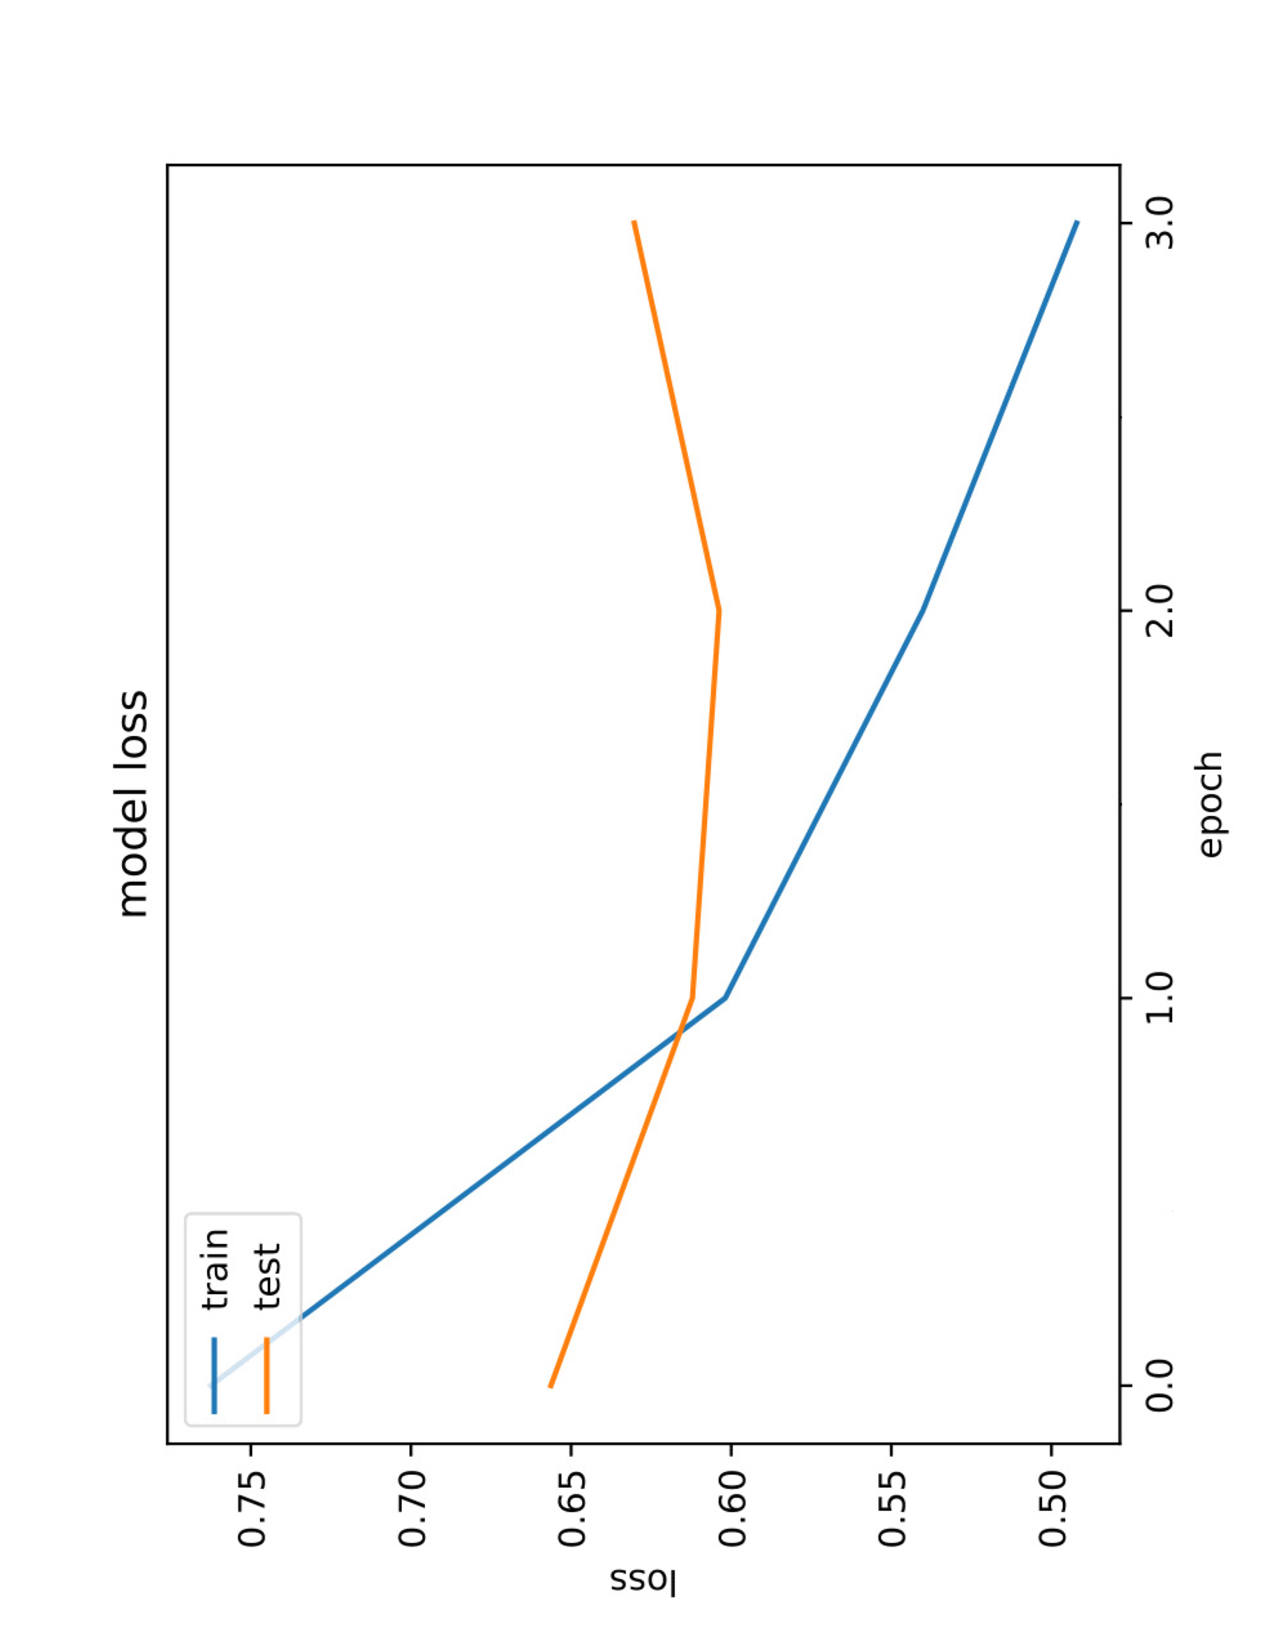
\includegraphics[width=70mm,scale=0.5]{gru_loss.pdf}
    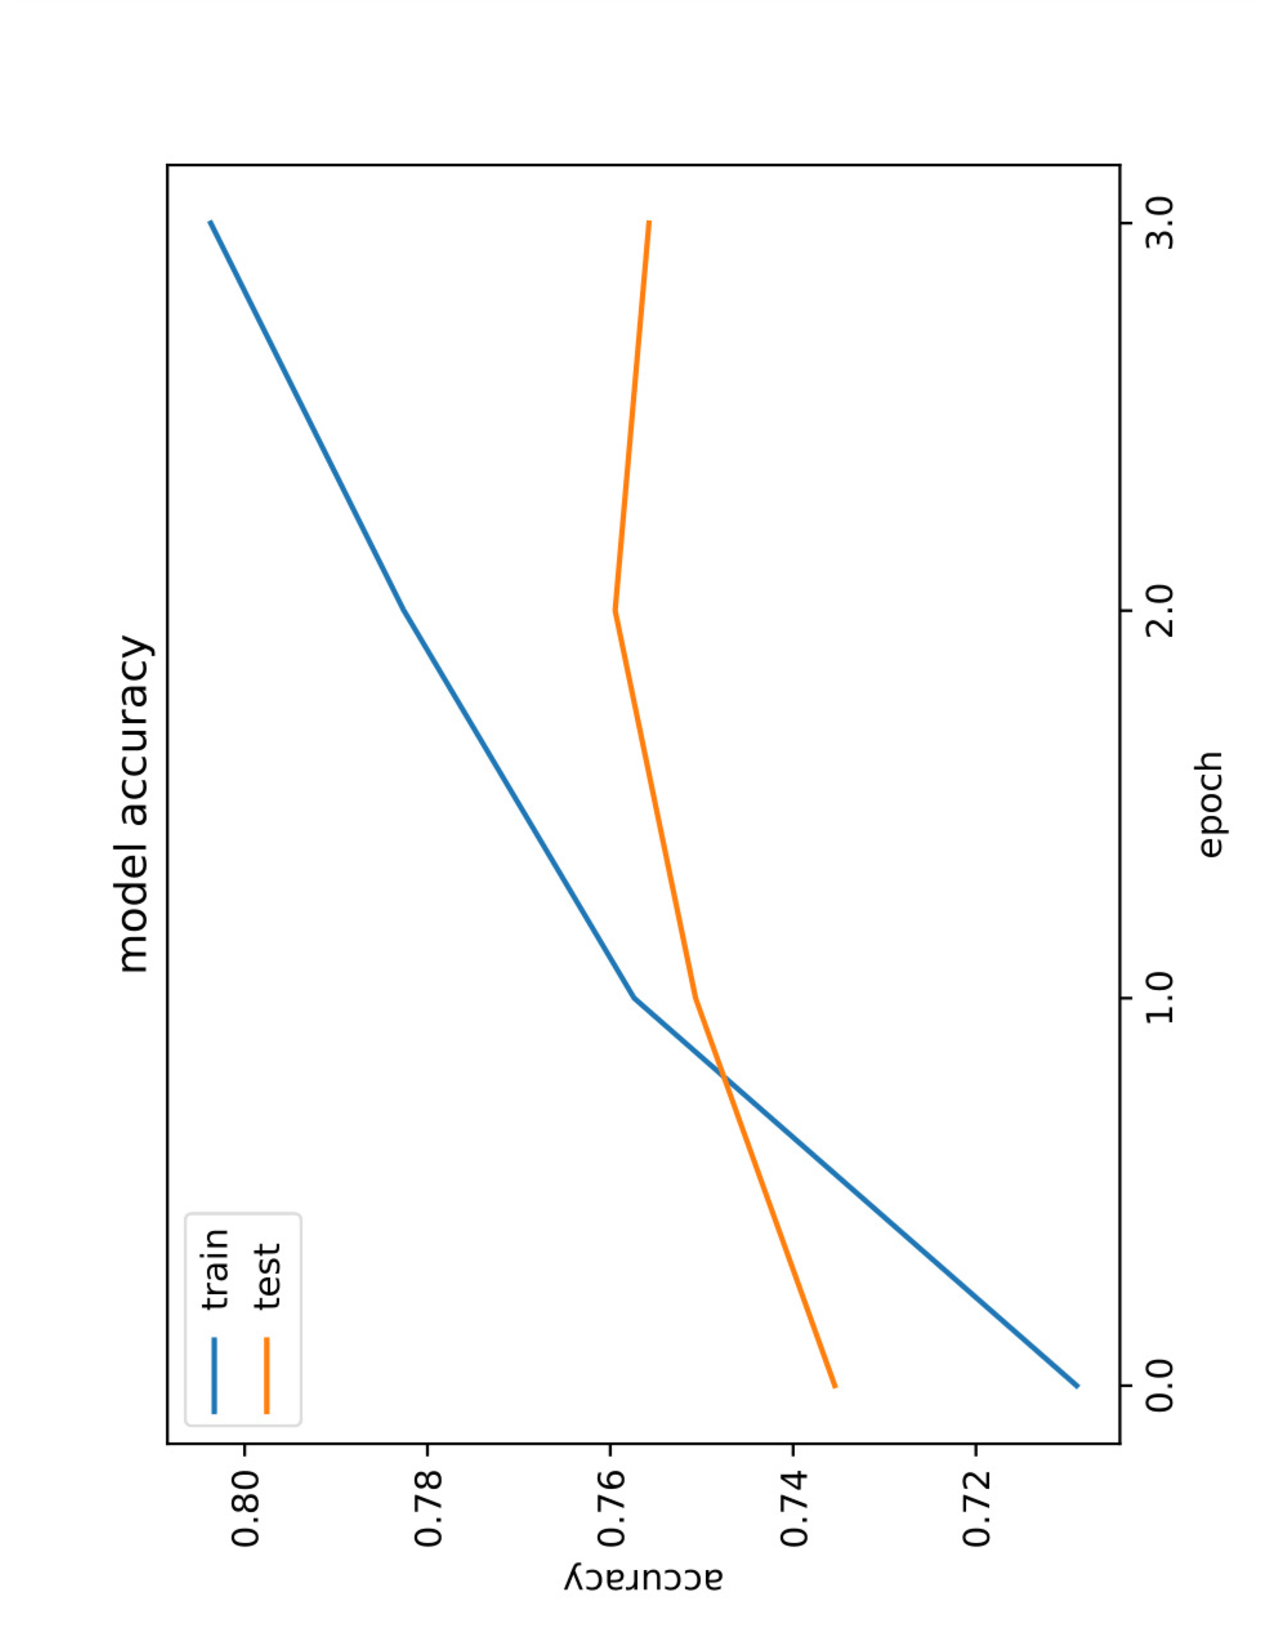
\includegraphics[width=70mm,scale=0.5]{gru_accuracy.pdf}
    \caption{GRU model loss and accuracy}
    \label{fig:gru}
\end{figure}
\begin{figure}[h!]
    \centering
    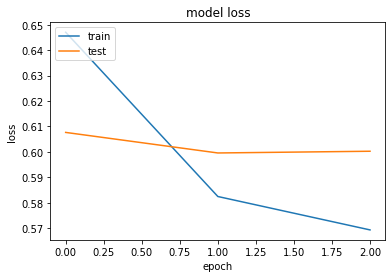
\includegraphics[width=70mm,scale=0.5]{trans_loss.png}
    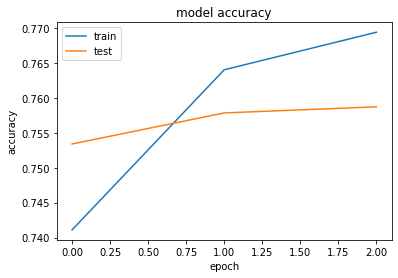
\includegraphics[width=70mm,scale=0.5]{trans_acc.png}
    \caption{TFBertModel model loss and accuracy}
    \label{fig:tr}
    \vspace{-0.5cm}
\end{figure}
\section{Conclusion}
With e-commerce becoming more popular, there will be higher demand for predicting programs on item rating, item recommendation and so on. Requirements for such programs would be fast, accurate and easy to adapt. This project uses GRU as the main layer to create a model that is capable of predicting user ratings with high accuracy by analyzing the most used word sequences from reviews. Through comparisons to other popular models, GRU is proven to yield good validation accuracy while using less training time and computational resources. Hence this model is a good starting point for building online recommendation systems. However, considering the accessibility of data in real life, there might be models that can make better use of what’s available, for instance combining reviewer and item information with the review contents to make more reliable predictions. These are certainly interesting areas to explore if there is more time for the project.

\medskip
\begin{thebibliography}{12} 
    \bibitem{imdb} 
    tf.keras.datasets.imdb.load\_data : TensorFlow Core v2.3.1
    \\\url{https://www.tensorflow.org/api\_docs/python/tf/keras/datasets/imdb/load\_data}
    \bibitem{gru} 
    Kostadinov, S. (2019, November 10). Understanding GRU Networks. Retrieved December 09, 2020, from
    \\\url{https://towardsdatascience.com/understanding-gru-networks-2ef37df6c9be}
    \bibitem{lstm} 
    Kang, E. (2017, September 01). Long Short-Term Memory (LSTM): Concept. Retrieved December 09, 2020, from 
    \\\url{https://medium.com/\@kangeugine/long-short-term-memory-lstm-concept-cb3283934359\#:~:text=LSTM\%20is\%20well\%2Dsuited\%20to,and\%20other\%20sequence\%20learning\%20methods.\&text=The\%20structure\%20of\%20RNN\%20is,hidden\%20Markov\%20model.}
    
    \bibitem{Textclassification}
    Text classification with an RNN \&nbsp;: \&nbsp; TensorFlow Core. (n.d.). Retrieved December 09, 2020, from
    \\\url{https://www.tensorflow.org/tutorials/text/text\_classification\_rnn}

    \bibitem{BERT}
    Jensen, E. (2020, August 25). Multi-Label, Multi-Class Text Classification with BERT, Transformer and Keras. Retrieved December 09, 2020, from
    \\\url{https://towardsdatascience.com/multi-label-multi-class-text-classification-with-bert-transformer-and-keras-c6355eccb63a}

    \bibitem{BERTpros}
    Horev, R. (2018, November 17). BERT Explained: State of the art language model for NLP. Retrieved December 09, 2020, from
    \\\url{https://towardsdatascience.com/bert-explained-state-of-the-art-language-model-for-nlp-f8b21a9b6270}

    \bibitem{trans}
    Maxime. (2020, March 05). What is a Transformer? Retrieved December 09, 2020, from
    \\\url{https://medium.com/inside-machine-learning/what-is-a-transformer-d07dd1fbec04}

    \bibitem{emd}
    Ruizendaal, R. (2020, June 02). Deep Learning \#4: Why You Need to Start Using Embedding Layers. Retrieved December 09, 2020, from
    \\\url{https://towardsdatascience.com/deep-learning-4-embedding-layers-f9a02d55ac12}

    \bibitem{graph}
    Admin. (2018, January 17). Apple release \'Turi Create\' Machine Learning Framework on Github. Retrieved December 09, 2020, from
    \\\url{https://todobi.com/apple-release-turi-create-machine/}
    % \\\url{https://towardsdatascience.com/deep-learning-4-embedding-layers-f9a02d55ac12}
    % \\\url{https://apple.github.io/turicreate/docs/api/generated/turicreate.recommender.create.html#turicreate.recommender.create}

    \end{thebibliography}

\end{document}
